\section{ステアリング、速度の制御}
  ロボカーがコースを走る際,直進コースでは機体を安定させ可能な限り速く走らせ,カーブに差し掛かったときにはステアリングとステアリングのための減速が必要である.特に,カーブを曲がりきるためにはどれだけのステアリング角と速度にすべきか,またその目標角度に追従させるためにはどのような制御系を構成する必要があるのかを考えなければならない.ここでは,ステアリング角と速度の目標値生成および制御方法について説明する.
 
 
\subsection{RCサーボモータ}
  ロボカーのステアリング角はRCサーボモータの角度により決められる.すなわち,各時点でのRCサーボモータへの目標角度生成と,その目標値に追従させるための制御方法を考える必要がある.

\subsubsection{目標値生成}
  本レースで走行させるロボカーは,機体の左右側面に設置された距離センサにより左右のコースの壁との距離を検出し,その距離の差に応じてステアリング角を変更させる.例えば,右側の壁との距離が左側の壁との距離より大きければステアリング角を時計回り方向に回転させる.ロボカーが直進コースを走行するときに比べ,カーブに差しかかったときとでは\refig{steering_compa}のように左右の壁との距離の差が大きくなる.すなわち,この距離の差が小さいときにはRCサーボモータの角度は小さくなり機体を進行方向に向かせるようにふるまい,大きくなるほど角度を大きくすることでカーブに差しかかった場合に必要なステアリング角を実現することができる.また,機体をコースの中央に位置させるようにステアリングを行わせることができる.
  
  ここで,RCサーボモータはPWM信号に対し\refig{RC_pulse}のような特性をもつ.RCサーボモータでのPWM信号の周期は$16〜23\unit{msec}$であり,その周期中のパルス幅の大きさに比例して角度が決まることがわかる.この特性より,パルス幅$W\unit{msec}$に対して目標角度$\theta_{r}=f(W)\unit{\deg}$とおく.また,左右の壁との距離の差に比例して目標角度を大きくしていくと,距離の差が小さいときに過剰なステアリングを行ってしまうことが考えられる.これが起こると,機体がコースの中央に位置し直進方向を向いているにもかかわらず小さな距離の差に反応してしまい機体の動きを不安定化させてしまう.よって,距離の差の大きさに応じてステアリング角の変化を大きくし,最大角度を超えないようにする必要があるためシグモイド関数$\sigma_{a}(x) $を用いた次式で目標角度$\theta_{r} $を生成することにした.

\begin{equation}  
  \theta = f(W) =f(1.5-2\cdot0.6(\sigma_{a}(x)-0.5)), 
  \sigma_{a}(x)=\frac{1}{1+e^{-ax}}
\end{equation}
ここで,$ a$は定数であり,$ x$は機体の左右のセンサの値の差である.シグモイド関数$\sigma_{a}(x) $は,この式は左右のセンサの値の差によりPWM信号のパルス幅を変えることで目標角度$\theta_{r} $を決定している.\refig{RC_pulse}に示したように,左右のセンサの値の差がなければ$x=0\unit{\deg}$となりパルス幅は$1.5\unit{msec}$となって目標角度$\theta_{r}$は$0\unit{\deg}$となる.右のセンサの値が左のセンサの値より大きい場合を正とすれば,RCサーボモータの角度は右の壁との距離の方が大きくなると時計回りに大きくなり,左の壁との距離のほうが大きくなると反時計回りに大きくなる.定数$a$はシグモイド関数の変化の速さにかかわり,試走実験を通して適切な値とする必要がある.

\subsubsection{構造}
  RCサーボモータは内部でフィードバック制御が行われている.その構造は\refig{RC_construction}に示すとおりである.目標角度に対応するPWM信号を入力すると内部で目標値に追従するように制御が行われる.よって,RCサーボモータの制御については制御系については考えず,目標角度を決めるだけとした.

\begin{figure}[htb]

  \centering
    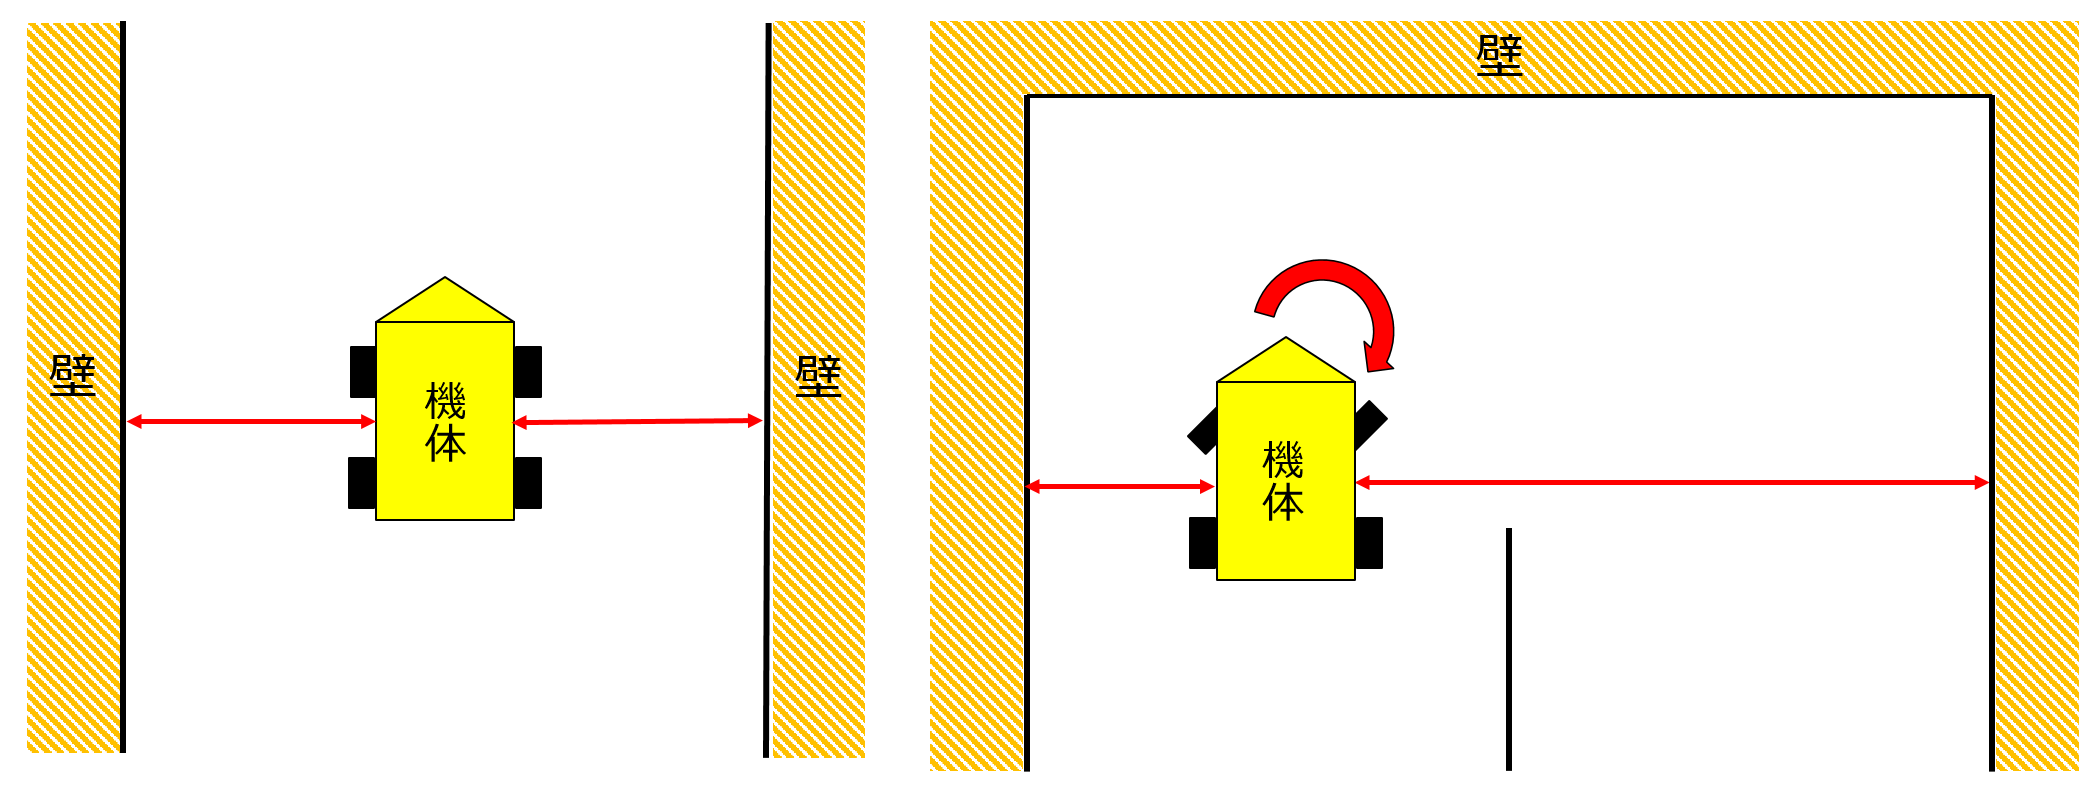
\includegraphics[width=0.7\hsize]{picture/eps/steering_compa.eps}
  \caption{左右の壁との距離の差によるステアリング}
  \label{fig::steering_compa}
\end{figure}  

\begin{figure}[htb]

  \centering
    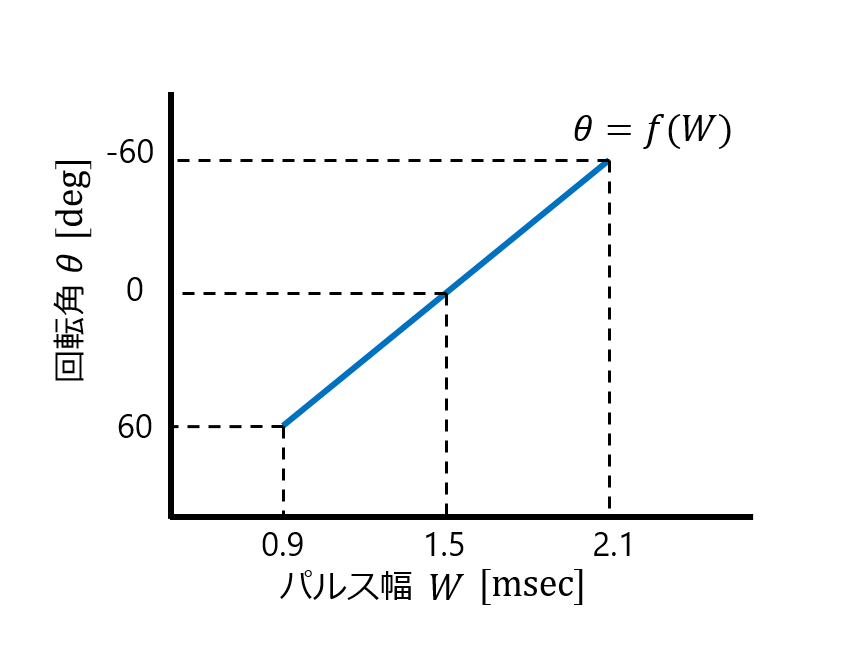
\includegraphics[width=0.5\hsize]{picture/eps/RC_pulse.eps}
  \caption{PWM信号のパルス幅とRCサーボモータの角度の関係}
  \label{fig::RC_pulse}
\end{figure} 
 
 \begin{figure}[htb]

  \centering
    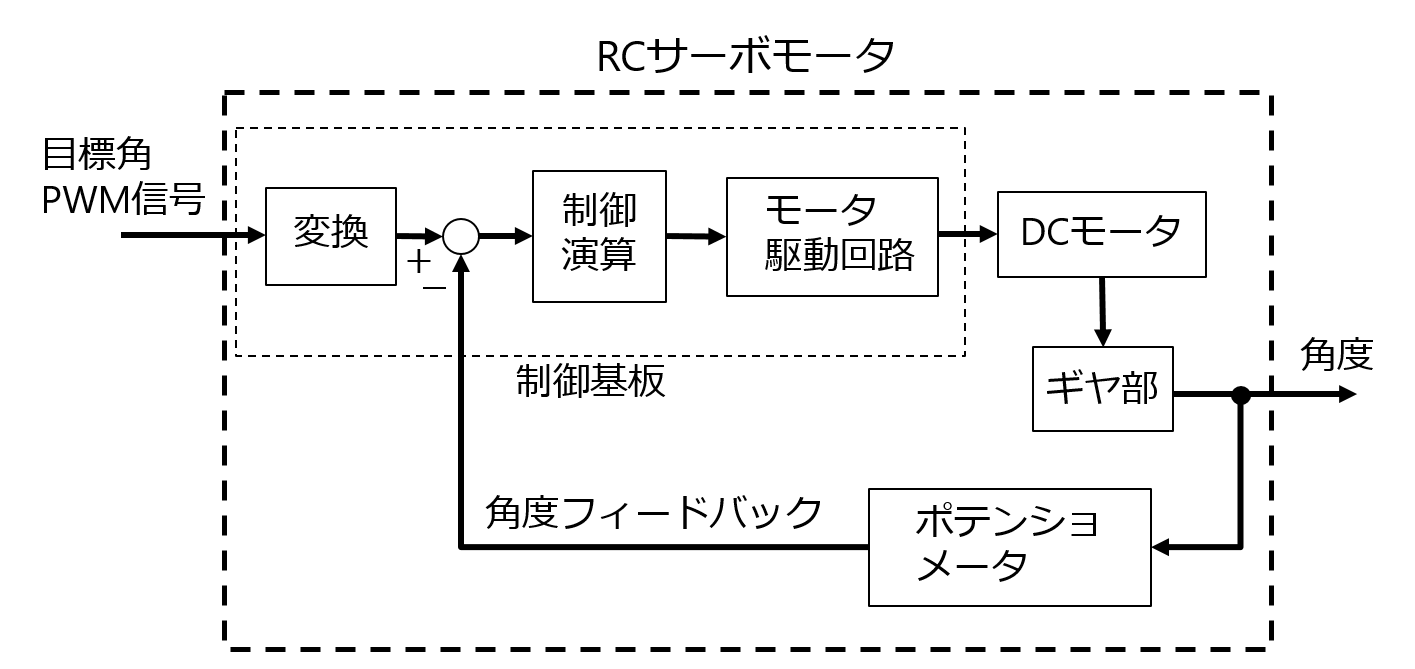
\includegraphics[width=0.6\hsize]{picture/eps/RC_construction.eps}
  \caption{RCサーボモータの制御系}
  \label{fig::RC_construction}
\end{figure} 

 \begin{figure}[htb]

  \centering
    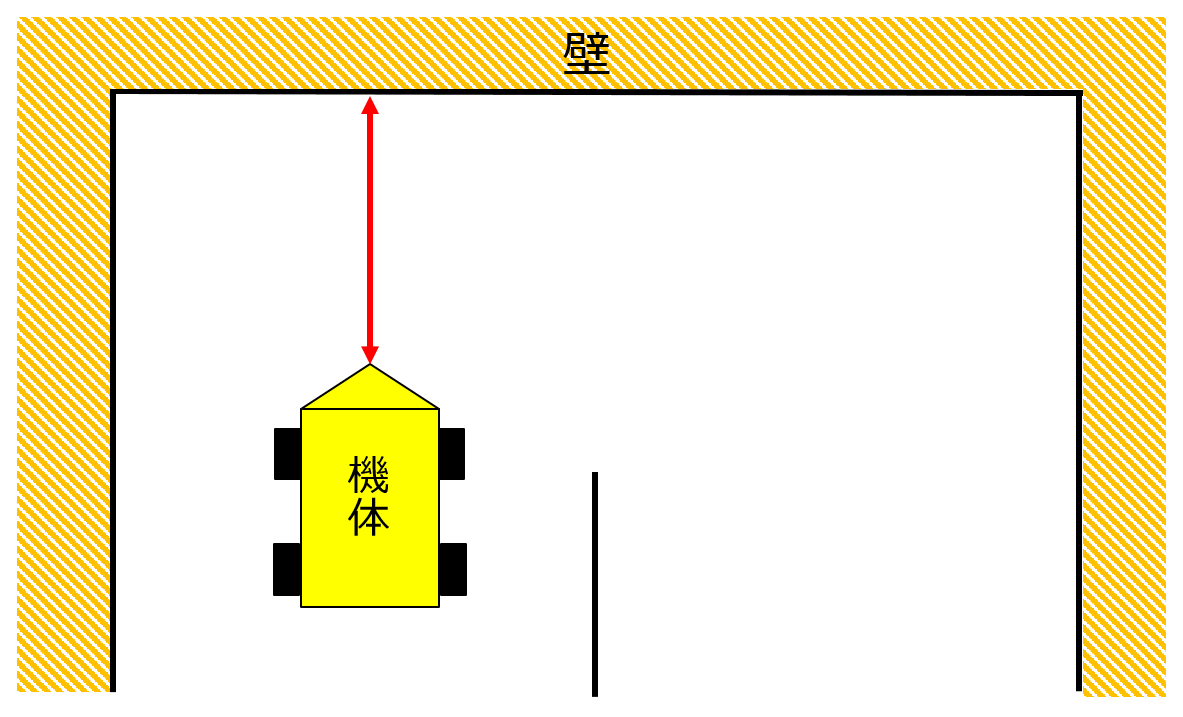
\includegraphics[width=0.4\hsize]{picture/eps/speed_wall.eps}
  \caption{前方の壁との距離に対する速度}
  \label{fig::speed_wall}
\end{figure}

\begin{figure}[htb]
  \centering
    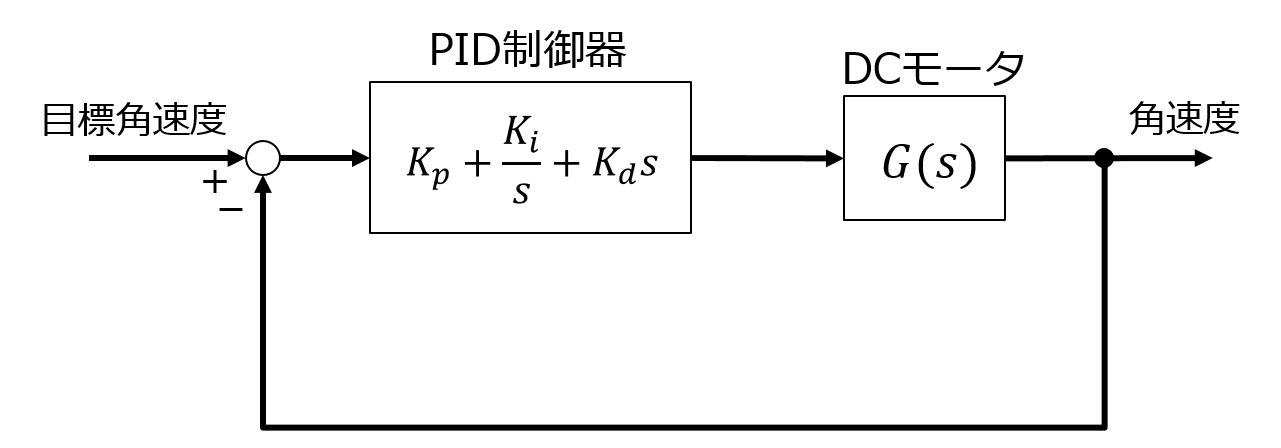
\includegraphics[width=0.5\hsize]{picture/eps/PID_control.eps}
  \caption{DCモータの制御系}
  \label{fig::PID_control}
\end{figure}

\clearpage
\subsection{DCモータ}
 ロボカーの速度はDCモータの回転角速度により決められる.すなわち,各時点でのDCモータへの目標角速度生成と,その目標値に追従させるための制御方法を考える必要がある.


\subsubsection{目標値生成}
 カーブを曲がりきるためには,ステアリングに余裕をもたせる速度が必要である.本レースで走行させるロボカーは,車体の正面に設置されたToFセンサにより前方の壁との距離を検出し,その距離に応じて速度を変化させる.\refig{speed_wall}のようにカーブに差しかかれば正面のコースの壁との距離は小さくなる.すなわち,正面のコースの壁との距離が小さくなるほどDCモータの角速度を小さくすることで,カーブでの減速を実現することができる.壁との距離に比例して目標角速度を生成すると,壁との距離が大きくなるほどDCモータの角速度が大きくなりモータの最大角速度まで大きくなってしまう.DCモータの角速度が最大の状態でロボカーを走らせると,消費電力が大きくなり電源の消耗が速くなる,機体がモータの回転に耐えられないなどの問題が生じる.この問題を解消するためには最大角速度をある値までに抑え,前方の壁との距離が一定以上になるとそれ以上角速度が上がらないようにする必要がある.なおかつ,壁との距離が小さくなれば速度を落としたいので,DCモータの角速度の目標値生成には,RCサーボモータと同様にシグモイド関数$\sigma_{a}(x)$を用いることにした.指定する最大角速度を$\omega_{max}\unit{rad/s} $とすれば,DCモータへの目標角速度$\omega_{r}\unit{rad/s}$は次式で生成される.

\begin{equation}
 \omega_{r}=2\omega_{max}(\sigma_{a}(x)-0.5), 
 \sigma_{a}(x)=\frac{1}{1+e^{-ax}}
\end{equation}

ここで,$a$は定数であり,$x$は前方のセンサの値である.シグモイド関数$\sigma_{a}(x)$は前方の壁との距離に対し増減する.この式を与えれば,壁との距離がどれだけ離れても目標角速度$\omega_{r}\unit{rad/s}$は指定最大角速度$\omega_{max}\unit{rad/s}$に抑えられ,電力消費を抑えることができる.定数$a$はシグモイド関数の変化の速さに関わり,試走実験を通して適切な値に決める必要がある.
\subsubsection{制御系}
  DCモータの制御系は,\refig{PID_control}に示すようにPID制御器を用いた閉ループ系で構成する.PID制御器を用いるのは,DCモータの角速度を目標角速度へ速やかに安定して到達させるためである.$G(s)$はDCモータの入力電圧から出力角速度への伝達関数であり,実験により求める必要がある.これはDCモータの入力電圧に対する出力角速度の応答を同定することで求められる.またPID制御器中の$K_{p}$,$K_{i}$,$K_{d}$は順に比例ゲイン,積分ゲイン,微分ゲインである.求めた伝達関数$G(s)$のボード線図から,ゲイン余裕,位相余裕などが適切な値になるように,また機体が想定通りの動きをするようにこれらのゲインを調節し,決定する必要がある.
